\chapter{Measures of Symmetry}%!chapter
\section{Skewness}
\textbf{Definition} An absolute frequency distribution is said to be skewed if it lacks symmetry.
- In other words, coeficient of skewness is a measure of symmetry of the distribution of a random variable.
- Skewness of data is measured by the pearsonian coeficient of skewness given by
\begin{equation}
    SK_p = \frac{\mu - mode}{\delta}
\end{equation}
- If the mode cannot be readily determined then we may employ a relationship among the mean, median and mode, given by
\begin{equation}
    \mu - mode = 3(\mu - median)
\end{equation}
to obtain
\begin{equation}
    SK_p = \frac{3(\mu - median)}{\delta}
\end{equation}
- For sample data, we can use $SK_p = \frac{3(\mu - median)}{\delta}$

- When $SK_p = 0$, it means $X's$ absolute frequency distribution is symetrical about the mean
- when $SK_p > 0$ it implies that the distribution of $X$ is skewed to the right ie. It has a longer tail on the right hand side of mean.
- when $SK_p < 0$ it means that the distribution of $X$ is skewed to the left ie. It has a longer tail on the left hand side of mean compared to the right.

\hbox{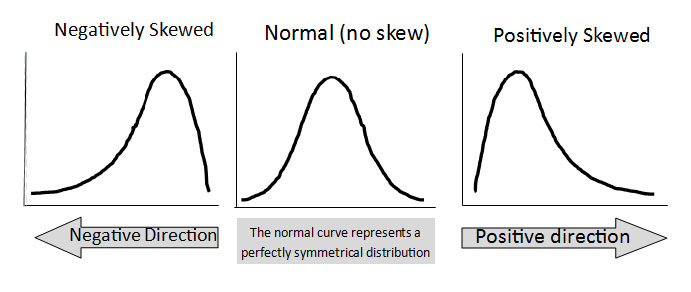
\includegraphics[width=\textwidth]{measure-of-skewness.jpg}}
- An alternative formula for computing skewness is through Quartiles. The Bowley's Coefiecient of skewness is given by
\begin{equation}
    SK_b = \frac{(Q_3 - Q_2)-(Q_2 - Q_1)}{Q_3 - Q_1}
\end{equation}
if $Q_2 - Q_1 = Q_3 - Q_2$, then the distribution is symetrical.
- if $Q_2 - Q_1 > Q_3 - Q_2$, the distribution is negatively skewed or skewed to the left.
- if $Q_2 - Q_1 < Q_3 - Q_2$, the distribution of $X$ is skewed to the right or is positively skewed.
\section{Kurtosis}
- Kurtosis refers to how flat or sharp the peak of the absolute frequency distribution happens to be.
- Both quantities are independent if units or dimensionless.
- The coeficient of kurtosis is estimated by
\begin{equation}
    K = \frac{\left(\frac{Q_3 - Q_1}{2} \right)}{P_{90} - P_{10}}
\end{equation}

where the numerator $QD = \frac{(Q_3 - Q_1)}{2}$ is called quartile deviation, which measures half the distance between the 1st and 3rd quartiles. While $P_{90}$ is $90^{th}$ percentile and $P_{10}$ is $10^{th}$ percentile.

\hbox{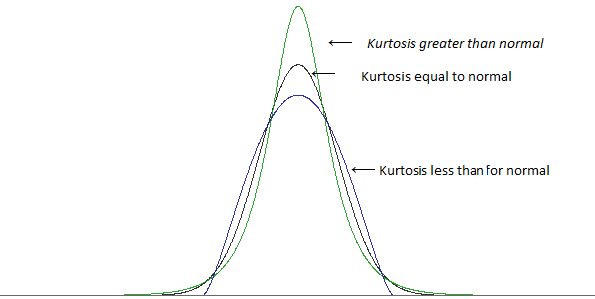
\includegraphics[width=\textwidth]{kurtosis.png}}
\newpage
%end of chapter
